\documentclass[a4paper,12pt]{article}
%% My standard included packages
%\pdfoutput=1 % if your are submitting a pdflatex (i.e. if you have
%             % images in pdf, png or jpg format)
%\usepackage{jcappub} % for details on the use of the package, please
%                     % see the JCAP-author-manual
%\usepackage[T1]{fontenc} % if needed

\usepackage{setspace}           % Allows easy changes to line spacing 
\usepackage{graphicx}           % Allows including of graphics files
\usepackage{amsmath}            % Additional math capabilities
\usepackage{marginnote}         % Used with todonotes package
\usepackage{datetime}           % Allows formatting of date and time
\newcommand {\be}{\begin{equation}}
\newcommand {\ee}{\end{equation}}
\usepackage[toc,page]{appendix}
\usepackage{cancel}

\usepackage{enumitem} 
\usepackage{listings}
\usepackage{amsmath}
\usepackage{graphicx}% Use pdf, png, jpg, or eps� with pdflatex; use eps in DVI mode
\usepackage{caption}
\usepackage{subcaption}
          % List formatting commands
\setlist{noitemsep}             % Remove space between list items 
%\usepackage{subfigure}          % Create numbered and captioned subfigures
\usepackage{rotating}           % Create landscape tables and figures
\usepackage[dvipsnames]{xcolor} % Refer to colors by name
\usepackage[colorlinks=true,urlcolor=blue,linkcolor=blue,citecolor=Black]{hyperref}           % URLS and hyperlinks
%\usepackage{hyperref}           % URLS and hyperlinks
\usepackage{float}              % Activate [H] option to place figure HERE
\usepackage[numbers]{natbib}
\usepackage{versionPO}          % Include text conditionally
\usepackage{caption}
%\usepackage[utf8]{inputenc}
%\usepackage[nottoc]{tocbibind}
\lstset{basicstyle=\ttfamily,
  showstringspaces=false,
  commentstyle=\color{red},
  keywordstyle=\color{blue}
}
% These next lines allow including or excluding different versions of text
% using versionPO.sty
\includeversion{notes}		% Include notes?
%\excludeversion{notes}
\excludeversion{comment}
\includeversion{links}          % Turn hyperlinks on?
\excludeversion{submit}		% Format for conference submission?
\includeversion{toc}		% Include table of contents?
%\graphicspath{{./Results1-Perihelionadvance}}

% Turn off hyperlinking if links is excluded
\iflinks{}{\hypersetup{draft=true}}

% Notes options
\ifnotes{%
\usepackage[margin=1in,paperwidth=10in,right=2.5in]{geometry}%
\usepackage[textwidth=1.4in,shadow,colorinlistoftodos]{todonotes}%
}{%
\usepackage[margin=1in]{geometry}%
\usepackage[disable]{todonotes}%
}

% Allow todonotes inside footnotes without blowing up LaTeX
% Next command works but now notes can overlap. Instead, we'll define 
% a special footnote note command that performs this redefinition.
%\renewcommand{\marginpar}{\marginnote}%

% Save original definition of \marginpar
\let\oldmarginpar\marginpar
% Workaround for todonotes problem with natbib (To Do list title comes out wrong)
\makeatletter\let\chapter\@undefined\makeatother % Undefine \chapter for todonotes
% Packages included specifically for this document.
\usepackage{texintro}           % Document-specific definitions
\usepackage{tocvsec2}           % More flexible formatting of table of contents
\usepackage{bibentry}           % Print full citation in text
\nobibliography*                                % Allow use of \bibentry command
\usepackage{tikz}             % Already included by todonotes
\usetikzlibrary{matrix}
\usepackage[retainorgcmds]{IEEEtrantools}  % Equation formatting. Option needed to
                                           % allow enumitem to work.

% Workaround for todonotes problem with natbib (To Do list title comes out wrong)
% If you're including tocvsec2, do so before this command.
\makeatletter\let\chapter\@undefined\makeatother % Undefine \chapter for todonotes.

% Number paragraphs and subparagraphs and include them in TOC
\setcounter{tocdepth}{2}

\usepackage[affil-it]{authblk} 
\usepackage{etoolbox}
%\usepackage{lmodern}
%\renewcommand\Authfont{\fontsize{12}{14.4}\selectfont}
%\renewcommand\Affilfont{\fontsize{9}{10.8}\itshape}
%\renewcommand\Authfont{\fontsize{12}{15}\selectfont}
%\renewcommand\Affilfont{\fontsize{9}{11}\itshape}
\definecolor{astral}{RGB}{46,116,181}
%\subsectionfont{\color{astral}}
%\sectionfont{\color{astral}}
%\usedate{31 August}                         % Use usual LaTeX date layout
%\date{ $1^{th}$ September, 2017}
%\title{\color{BlueViolet}\Huge{On the accuracy of approximated geodesic equations and different potentials with different numerical methods } }
\title{\color{BlueViolet}\Huge{K-essence field equation}}
%\vskip 2em
\author{Farbod Hassani}
%\thanks{Email:\href{mailto:farbod.hassani@unige.ch}{{farbod.hassani@unige.ch}}}  \thanks{Homepage: \href{http://www.farbod-hassani.com}{farbod-hassani.com}}}
%\affil{D\'epartement de Physique Th\'eorique and Center for Astroparticle Physics, Universit\'e de Gen\'eve,
%24 quai Ansermet, CH-1211 Gen\'eve 4, Switzerland}

%{farbod-hassani.com}} }
%\newcommand*{\TitleFont}{%     \usefont{\encodingdefault}{\rmdefault}{b}'%     \fontsize{18}{16}%    \selectfont}
%\title{\TitleFont Halo finder}
%\author[1]{{Farbod Hassani} \thanks{ \url{farbod.hassani@gmail.com}
%}
%\thanks{farbod-hassani.com}}
%\author[2]{Author E\thanks{E.E@university.edu}}
%\affil[1]{D\'epartement de Physique Th\'eorique and Center for Astroparticle Physics, Universit\'e de Gen\'eve,
%24 quai Ansermet, CH-1211 Gen\'eve 4, Switzerland}
%\emailAdd{farbod.hassani@gmail.com}
%\affil[2]{Department of Mechanical Engineering, \LaTeX\ University}
      %\begin{abstract}
%This is abstract text: This simple document shows very basic features of \LaTeX{}.
%\lstset { %
%    language=C++,
%    %backgroundcolor=\color{black!5}, % set backgroundcolor
%    basicstyle=\footnotesize,% basic font setting
%}
\begin{document}

  \maketitle
  \tableofcontents

  \flushbottom
\section{Theory} 
The most general action for a scalar field coupled to Einstein gravity is;
\be
S=\frac{1}{16 \pi G} \int \sqrt{-g} R d^4 x + \int \sqrt{-g} P (X, \varphi) d^4 x
\ee
The metric convention is $(-,+,+,+)$ and $X=- \frac{1}{2}  g^{\mu \nu}\partial _\mu \phi \partial_\nu \phi$. We  assume the scalar action as a matter sector which contributes to stress energy tensor,
\be
T^{\mu\nu}\equiv \dfrac {+2}{\sqrt {-g}}\dfrac {\delta \mathcal{ L}}{\delta g_{\mu\nu}}=\dfrac {2}{\sqrt {-g}}\dfrac {\delta \left[ \sqrt {-g}P\left( X,\varphi \right) \right] }{\delta g_{\mu\nu}}
=
\dfrac {2}{\sqrt {-g}}[- \dfrac {1 }{2 \sqrt{-g}} \frac{\delta g}{\delta g_{\mu\nu}}P\left( X,\varphi\right) +\dfrac {\delta P\left( X,\varphi\right) }{\delta g_{\mu\nu}}\sqrt {-g}]
\ee
According to appendix \ref{A1},
\be
\dfrac {\delta \sqrt {-g}}{\delta g_{\mu\nu}}=\dfrac {-1}{2\sqrt {-g}}\dfrac {\delta g}{\delta g_{\mu\nu}}=\dfrac {-1}{2\sqrt {-g}}\dfrac {g\delta g_{\mu\nu}g^{\mu\nu}}{\delta g_{\mu\nu}}=\dfrac {\sqrt {-g}}{2}g^{\mu\nu}
\ee
\be
T^{\mu\nu}=2\dfrac {\delta P\left( X,\varphi\right) }{\delta g_{\mu\nu}} + g^{\mu\nu}P\left( X,\varphi\right)
\ee
\be
T_{\rho \sigma}=g_{\mu \rho} g_{\nu \sigma} T^{\mu \nu}= \Big[ 2 g_{\mu \rho} g_{\nu \sigma}  \dfrac {\delta P\left( X,\varphi\right) }{-g_{\mu \rho'} g_{\nu \sigma'}  \delta g ^{\sigma' \rho'}} + g_{\mu \rho} g_{\nu \sigma}  g^{\mu\nu}P\left( X,\varphi\right) \Big]= -2\dfrac {\delta P \left( X,\varphi\right) }{\delta g^{\rho \sigma}}+g_{\rho \sigma}P\left( X,\varphi\right)
\ee
Where we have used $\delta g_{\mu \nu}= - g_{\mu \rho} g_{\nu \sigma} \delta g^{\rho \sigma}$.
\begin{align}
X=-\dfrac {1}{2}g^{\mu\nu}\partial_{\mu}\varphi\partial_{\nu}\varphi \longrightarrow  \delta X=-\dfrac {1}{2}\delta g^{\mu\nu}\partial_{\mu}\varphi\partial_{\nu}\varphi-\dfrac {1}{2}g^{\mu\nu}\partial_{\mu}\delta \varphi\partial_{\nu}\varphi-\dfrac {1}{2}g^{\mu\nu}\partial_{\mu}\varphi\partial_{\nu}\delta\varphi
\end{align}
so,
\be
\dfrac {\partial X}{\partial g^{\mu\nu}}=-\dfrac {\partial_{\mu}\varphi\partial_{\nu}\varphi}{2}
\ee
\be
\dfrac {\delta P}{\delta g^{\mu\nu}}=\dfrac {\partial P}{\partial X}\dfrac {\partial X}{\partial g^{\mu\nu}}+ \cancel{\dfrac {\partial P}{\partial\varphi}\dfrac {\partial\varphi}{\partial g^{\mu\nu}}}=\dfrac {\partial P}{\partial X}\dfrac {\partial X}{\partial g^{\mu\nu}}=-\dfrac {\partial_{\mu}\varphi\partial_{\nu}\varphi}{2}P_{,X}
\ee
\be
T_{\mu\nu}=g_{\mu\nu}P\left( X,\varphi\right) +P_{,X}\partial_{\mu}\varphi\partial_{v}\varphi \; , \;
T_{\mu\nu}=\left( \rho+p\right) u_{\mu}u_{\nu}+p g_{\mu\nu}
\ee
\be
u_{\mu}=\dfrac {\partial_{\mu}\varphi}{\sqrt {-\partial_{\mu}\varphi\partial^{\mu}\varphi}}\rightarrow u_{\mu}=\dfrac {\partial_{\mu}\varphi}{\sqrt {2X}} , \rho=2XP_{,X}-P \; , \; p=P  \label{eq10}
\ee
We assume that field is a monotonic function of time in background which is perturbed in each constant time hypersurfaces
\be
\varphi_{0}\left( \tau+\pi\left( \tau,\overrightarrow {x}\right) \right) =\varphi_{0}\left( \tau \right) +\dfrac {\partial\varphi_{0}}{\partial  \tau }\pi+\dfrac {\partial^{2}\varphi_{0}}{2\partial^{2} \tau}\pi^{2}+\ldots
\ee
We can choose $\varphi_0(\tau)=\tau$ for simplicity, using the following ansatz for the metric,
\be
g_{\mu\nu}=a(\tau)^2 \Big [-e^{2\Psi}d\tau^{2}+ e^{-2\Phi}dr^{2} \Big]
\ee
where $\tau$ is the conformal time.
\be
\delta g^{(1)}_ { 00}=-2\, a^2 \Psi \, \; \; , 
\delta g^{(1)}_{ij}= -2 a^{2} \Phi \delta_{ij}
\ee
Where $\delta g^{(1)}_ { 00}$ means the first order metric in pertubations.  The inverse of metric is defined as following,
\be
g^{\mu\nu}=\frac{1}{a^2} \Big [-e^{-2\Psi}d\tau^{2}+e^{2\Phi}dr^{2}  \Big ]
\ee
\be
\delta g_{(1)}^{00}=+\frac{2\Psi}{a^2} \, \; \; , 
\delta g_{(1)}^{ij}= + \frac{2\Phi \delta^{ij} }{a^2}
\ee
We have,
\be
X=\dfrac {-1}{2}g^{\mu\nu}\partial_{\mu}\left( \tau+\pi\right) \partial_{\nu}\left( \tau+\pi\right) 
\ee
We expand X perturbatively,
\be
X=\overline {X}+\delta X_{1}+ \delta X_{2}+\ldots
\ee
\be
\overline {X}=-\dfrac {1}{2}\bar{g}^{00}\partial_{0} \tau \partial_{0} \tau=+\dfrac {1}{2 a^2}\\
\ee
\be
\delta X_{1}=-\dfrac {1}{2}\delta g_{(1)}^{00}\partial_{0} \tau \partial_{0} \tau-\dfrac {1}{2} \bar{g}^{00}\partial_{0} \tau \partial_{0}\pi-\dfrac {1}{2} \bar{g}^{00}\partial_{0}\pi\partial_{0} \tau-\dfrac {1}{2}\bar{g}^{ij}\partial_{i}\pi\partial_{j}\pi
\ee
\be
 \delta X_{1}=\frac{1}{a^2} \Big [-\Psi+{\pi'}- \frac{(\vec{\nabla} \pi)^2}{2 }  +O\left( \varepsilon^{2}\right) \Big]
\ee
We do not need to calculate $X_2$ since the energy momentum constraint adds at most one spatial derivative which does not change the second order terms to first order. So
\be
P\left(\varphi( \tau+\pi),\overline{X}+ \delta X_1+\delta X_2 \right) =\overline{P}\left( \varphi( \tau),\overline {X}\right) 
+ \cancel{\dfrac {\partial\overline {P}}{\partial \tau}} \pi+\dfrac {1}{2} \cancel{\dfrac {\partial^{2}\overline {P}}{\partial \tau^2}}\pi^{2}
+
\dfrac {\partial\overline {P}}{\partial\overline {X}}\delta X_1+\dfrac {1}{2}\dfrac {\partial P}{\partial X^{2}}\delta X_1^{2} +\dfrac {1}{2}\dfrac {\partial P}{\partial X^{2}}\delta X_2 + \mathcal{O}(\epsilon^3).
\ee
The term $\dfrac {\partial\overline {P}}{\partial \tau}$ cancels since  $\dfrac {\partial\overline {P}}{\partial \tau}=\dfrac {\partial\overline {P}}{\partial  {\varphi}} \dfrac{\partial {\varphi}}{\partial \tau}+ \dfrac {\partial\overline {P}}{\partial  {X}} \dfrac{\partial {X}}{\partial \tau} =0$. Because $\varphi$ and $\partial_{\mu} \varphi$ are independent variables not function of $\tau$. \\
The adiabatic sound speed ({\color{red}why?!}) is defined as below,
\be
%c^{2}_{s}\equiv \frac{\delta P}{\delta \rho} =\dfrac {\bar{P}_{,X} \delta X + \bar{P}_{,\varphi} \delta \varphi}{\bar{\rho}_{,X} \delta X  +\bar{\rho}_{,\varphi} \delta  \varphi}=\dfrac {\bar{P}_{,X}}{\bar{\rho}_{,X}}=\dfrac {\bar{P}_{,X}}{\bar{P}_{,X}+2\bar{X}\bar{P}_{,XX}} 
c^{2}_{s}\equiv \dfrac {\bar{P}_{,X}}{\bar{\rho}_{,X}}=\dfrac {\bar{P}_{,X}}{\bar{P}_{,X}+2\bar{X}\bar{P}_{,XX}} 
\ee
and 
\be
\Omega= \frac{\bar{\rho}}{3 M_{pl}^2 H^2}=\frac{{2\bar{X} \bar{P}_{,X}-\bar{P}}}{3 M_{pl}^2 H^2} \label{22}
\ee
Where we have used $ \rho=2XP_{,X}-P$
\be
\omega=\dfrac {\overline {P}}{\overline {\rho}}=\dfrac {\overline {P}}{2\overline {X} \, \overline{P}_{,X}-\overline {P}} \label{23}
\ee
So we can write the function $P$ and it derivative in terms of $\Omega$, $\omega$ and $c_s^2$,
\be
\bar{P}_{X}= a^2 \bar{P} (1+\frac{1}{\omega}) \; \; \; \; \;  \; \bar{P} _{,XX}=a^2  \bar{P}_{,X} \frac{1-c_s^2}{c_s^2} =a^4  \bar{P} (1+\frac{1}{\omega}) (\frac{1}{c_s^2} -1 )
\label{Pbarder}
\ee
So according to \ref{22} and \ref{23}\\
\be
\bar{P}=  3 M_{pl}^2 H^2 \Omega \, \omega = \frac{ 3 M_{pl}^2 \mathcal{H}^2 \Omega\, \omega }{a^2} \label{Pbar}
\ee
The relation between Hubble and conformal Hubble is;
\be
\mathcal{H} (\tau)=\frac{1}{a(\tau) }\frac{d a(\tau)}{d \tau }= \frac{1}{a(t) } \frac{d a (t) }{d t} \frac{d t }{ d\tau}= a H(t)
\ee
Now we can construct stress tensor up to first order in Gevolution's perturbation scheme,
\begin{align} \label{eqTmunuI}
T_{\mu \nu} &= P g_{\mu \nu} + P_{,X} \partial_{\mu} \varphi \partial_{\nu} \varphi \\ \nonumber & =(\bar{g}_{\mu \nu} + \delta g^{(1)}_{\mu \nu}) (\bar{P}+\bar{P}_{,X} \delta X_1) + (\bar{P}_{,X}+\bar{P}_{,XX} \delta X_1) \partial_{\mu} (\tau+ \pi) \partial_\nu (\tau+\pi)+ \ldots
\\ \nonumber & 
= \Big[ \bar{g}_{\mu \nu} \bar{P} 
+
 \bar{P}_{,X} \partial_{\mu} \tau \partial_{\nu} \tau \Big] \epsilon ^0 
+
\Big[ \bar{g}_{\mu \nu}  \bar{P}_{,X} \delta X_1 
+
 \delta g^{(1)}_{\mu \nu} \bar{P} 
 +
  \bar{P}_{,X}  \left ( \partial_{\mu} \pi \partial_{\nu} \tau  
  +
  \partial_{\mu} \tau \partial_{\nu} \pi  \right ) 
  +
   \delta X_1 \bar{P}_{,XX}   \partial_{\mu} \tau \partial_{\nu} \tau  
   +
    \bar{P}_{,X}   \partial_{\mu} \pi \partial_{\nu} \pi \nonumber \\ &
    +  \delta X_1 \bar{P}_{,XX}  \big(  \partial_{\mu} \tau \partial_{\nu} \pi  +   \partial_{\mu} \pi \partial_{\nu} \tau  \big)
    + \cancelto{\mathcal {O}(\epsilon^{2})}{\delta X_1 \bar{P}_{,XX}   \partial_{\mu} \pi \partial_{\nu} \pi  
   } \Big ] 
 \; \; \;+ \mathcal {O}(\epsilon^{2}) 
\end{align}
%\newpage
\section{$T_{00}$ component of energy momentum tensor}
According to previous equation $T_{00} $ component is,
\begin{align} \label{T00}
T_{00} &=
   \Big[ \bar{g}_{0 0} \bar{P} 
+
 \bar{P}_{,X} \partial_{0} \tau \partial_{0} \tau \Big] \epsilon ^0 
+
\Big[ \bar{g}_{0 0}  \bar{P}_{,X} \delta X_1 
+
 \delta g^{(1)}_{0 0} \bar{P} 
 +
  \bar{P}_{,X}  \left ( \partial_{0} \pi \partial_{0} \tau  
  +
  \partial_{0} \tau \partial_{0} \pi  \right ) 
  +
   \delta X_1 \bar{P}_{,XX}   \partial_{0} \tau \partial_{0} \tau 
   +
    \cancelto{\mathcal {O}(\epsilon^{2}) 
} { \bar{P}_{,X}  } \partial_{0} \pi \partial_{0} \pi  +   \cancelto{\mathcal {O}(\epsilon^{2})}  {2 \pi'   } \delta X_1  \bar{P}_{,XX}  \Big ]
%::::::::::::::::::::::::::::::::::::::::::::::::::::::::::::::::::::::::::::::::::::::::::::::::::::::::::::::::
%::::::::::::::::::::::::::::::::::::::::::::::::::::::::::::::::::::::::::::::::::::::::::::::::::::::::::::::::
  \nonumber
 \\
  &
  =
  [-a^2  \bar{P} 
+
 \bar{P}_{,X}  ] \epsilon ^0 
+
\Big[ - a^2 \bar{P}_{,X} \delta X_1 
-
 2 a^2 \Psi \bar{P} 
 +
 2 \bar{P}_{,X}   {\pi'}
  +
   \delta X_1 \bar{P}_{,XX} 
  \Big ] 
+ \mathcal {O}(\epsilon^{2}) 
%::::::::::::::::::::::::::::::::::::::::::::::::::::::::::::::::::::::::::::::::::::::::::::::::::::::::::::::::
%::::::::::::::::::::::::::::::::::::::::::::::::::::::::::::::::::::::::::::::::::::::::::::::::::::::::::::::::
  \nonumber
 \\
  &
  =
  [-a^2 \bar{P} 
+
a^2 \bar{P}  (1+\frac{1}{w}) ] \epsilon ^0 
+
\Big[ - a^4 \bar{P}  (1+\frac{1}{w})  \delta X_1 
-
 2 a^2  \Psi \bar{P} 
 +
 2  a^2 \bar{P}  (1+\frac{1}{w})  {\pi'}
  +
  a^4 \bar{P}  (1+\frac{1}{w}) (\frac{1}{c_s^2}-1) \,   \delta X_1 
   \Big ] 
+ \mathcal {O}(2) 
%::::::::::::::::::::::::::::::::::::::::::::::::::::::::::::::::::::::::::::::::::::::::::::::::::::::::::::::::
%::::::::::::::::::::::::::::::::::::::::::::::::::::::::::::::::::::::::::::::::::::::::::::::::::::::::::::::::
  \nonumber
 \\
  &
  =
 \frac{ a^2 \bar{P}}{w} \,\epsilon ^0 
+
\frac{ a^2\bar{ P}}{w}   \Big[ - a^2   (1+w)  \delta X_1 
-
 2   w \Psi
 +
 2  (1+w)  {\pi'}
  +
  a^2 (1+w) (\frac{1}{c_s^2}-1) \,   \delta X_1 
   \Big ] \epsilon^1
+ \mathcal {O}(\epsilon^{3/2}) 
%::::::::::::::::::::::::::::::::::::::::::::::::::::::::::::::::::::::::::::::::::::::::::::::::::::::::::::::::
%::::::::::::::::::::::::::::::::::::::::::::::::::::::::::::::::::::::::::::::::::::::::::::::::::::::::::::::::
  \nonumber
 \\
  &
  =
\frac{a^2 \bar{ P}}{w} \,\epsilon ^0 
+
\frac{a^2 \bar{ P}}{w}   \Big[  a^2 (1+w) (\frac{1}{c_s^2}- 2)  \delta X_1 
-
 2 w \Psi
 +
 2  (1+w)  {\pi'}
 \Big ] 
+ \mathcal {O}(\epsilon^{2}) 
%::::::::::::::::::::::::::::::::::::::::::::::::::::::::::::::::::::::::::::::::::::::::::::::::::::::::::::::::
%::::::::::::::::::::::::::::::::::::::::::::::::::::::::::::::::::::::::::::::::::::::::::::::::::::::::::::::::
  \nonumber
 \\
  &  
  =
3 M_{pl}^2 \mathcal{H}^2 \Omega  \,\epsilon ^0 
+
3 M_{pl}^2  \mathcal{H}^2 \Omega    \Bigg[  (1+w) (\frac{1}{c_s^2}- 2)  \Big[ -\Psi+{\pi'}-  \frac{(\vec{\nabla} \pi)^2}{2} \Big ]
-
 2 w \Psi
 +
 2  (1+w)  {\pi'}
 \Bigg ]
+ \mathcal {O}(\epsilon^{2})  
%::::::::::::::::::::::::::::::::::::::::::::::::::::::::::::::::::::::::::::::::::::::::::::::::::::::::::::::::
%::::::::::::::::::::::::::::::::::::::::::::::::::::::::::::::::::::::::::::::::::::::::::::::::::::::::::::::::
  \nonumber
 \\
  &
  =
3 M_{pl}^2  \mathcal{H}^2 \Omega \Bigg[  1+ \Psi \Big (- (1+w) (\frac{1}{c_s^2}- 2)-2 w  \Big ) + {\pi'} \Big ( (1+w) (\frac{1}{c_s^2}- 2 )+2 (1+w)   \Big)  - \frac{(\vec{\nabla} \pi)^2}{2}  \Big ( (1+w) (\frac{1}{c_s^2}- 2 )  \Big )
 \Bigg]
 %::::::::::::::::::::::::::::::::::::::::::::::::::::::::::::::::::::::::::::::::::::::::::::::::::::::::::::::::
%::::::::::::::::::::::::::::::::::::::::::::::::::::::::::::::::::::::::::::::::::::::::::::::::::::::::::::::::
   \nonumber
 \\
  &
  =
3 M_{pl}^2  \mathcal{H}^2 \Omega \Bigg[  1+ \Psi \Big (2 - \frac{1+w}{c_s^2}  \Big ) + {\pi'} \Big ( \frac{1+w}{c_s^2}   \Big)  - \frac{(\vec{\nabla} \pi)^2}{2}   \Big ( (1+w) (\frac{1}{c_s^2}- 2 )  \Big )
 \Bigg]+  \mathcal {O}(\epsilon^{2}) 
\end{align}
Where we have used \ref{Pbarder} and \ref{Pbar}.
Finaly the $T_{00}$ component is;
\be
T_{00}=  
3 M_{pl}^2   \mathcal{H}^2\Omega \Bigg[  1+ \Psi \Big (2 - \frac{1+w}{c_s^2}  \Big ) + {\pi'} \Big ( \frac{1+w}{c_s^2}   \Big)  -  \frac{(\vec{\nabla} \pi)^2}{2}   \Big ( (1+w) (\frac{1}{c_s^2}- 2 )  \Big )
 \Bigg]+  \mathcal {O}(\epsilon^{2}) 
\ee
\section{$T_{0i}$ component of energy momentum tensor}
According to the equation \ref{eqTmunuI} we can calculate $T_{0i}$ component of energy momentum tensor
\begin{align}
T_{\mu \nu} &
= \Big[ \bar{g}_{\mu \nu} \bar{P} 
+
 \bar{P}_{,X} \partial_{\mu} \tau \partial_{\nu} \tau \Big] \epsilon ^0 
+
\Big[ \bar{g}_{\mu \nu}  \bar{P}_{,X} \delta X_1 
+
 \delta g^{(1)}_{\mu \nu} \bar{P} 
 +
  \bar{P}_{,X}  \left ( \partial_{\mu} \pi \partial_{\nu} \tau 
  +
  \partial_{\mu} \tau \partial_{\nu} \pi  \right ) 
  +
   \delta X_1 \bar{P}_{,XX}   \partial_{\mu} \tau \partial_{\nu} \tau  
   +
    \bar{P}_{,X}   \partial_{\mu} \pi \partial_{\nu} \pi  + 
     \nonumber \\ &
    +  \delta X_1 \bar{P}_{,XX}  \big(  \partial_{\mu} \tau \partial_{\nu} \pi  +   \partial_{\mu} \pi \partial_{\nu} \tau \big ) \Big]
+ \mathcal {O}(\epsilon^{2}) 
%\label{eqTmunu}
\end{align}
So $T_{0i}$ reads;
\begin{align} \label{T0i}
T_{0 i} &
= \Big[ \cancel{\bar{g}_{0 i}} \bar{P} 
+
 \bar{P}_{,X} \partial_{0} \tau \partial_{i} \tau \Big] \epsilon ^0 
+
\Big[ \cancel{\bar{g}_{0 i}}  \bar{P}_{,X} \delta X_1 
+
 \delta g^{(1)}_{0 i} \bar{P} 
 +
  \bar{P}_{,X}  \Big( \partial_{0} \pi \cancel{ \partial_{i} \tau  }
  +
  \partial_{0} \tau \partial_{i} \pi  \Big ) 
  +
   \delta X_1 \bar{P}_{,XX}   \partial_{0} \tau  \cancel{\partial_{i} \tau  }
   +
     \delta X_1 \bar{P}_{,XX}   \partial_{0} \tau  \partial_{i} \pi
     \nonumber  \\&
  +
    {\bar{P}_{,X} } \partial_{0} \pi \partial_{i} \pi \; \;   \Big ]
+ \mathcal {O}(\epsilon^{2}) 
\nonumber 
\\ 
&
= [0] \epsilon ^0 
+
\Big[
 \delta g^{(1)}_{0 i} \bar{P} 
 +
  \bar{P}_{,X}   \partial_{0} \tau \partial_{i} \pi +  {\bar{P}_{,X} } \partial_{0} \pi \partial_{i} \pi + \delta X_1 \bar{P}_{,XX}    \partial_{i} \pi
  \Big ] 
+ \mathcal {O}(\epsilon^{2}) 
\nonumber 
\\ 
&
= 
3 M_{pl}^2 \mathcal{H}^2 \Omega \Bigg[
 w \, \frac{\delta g^{(1)}_{0 i} }{a^2}
 +
   (1+w )\,  \partial_{i} \pi + (1+w) \, \pi' \partial_{i} \pi  +(1+ w)(\frac{1}{c_s^2}-1)  \Big (-\Psi+ \pi' -\frac{(\vec{\nabla} \pi)^2}{2} \Big) \partial_{i} \pi 
   \Bigg ]
+ \mathcal {O}(\epsilon^{2}) 
%\label{eqTmunu}
\end{align}
Note that $T_{0i}=T_{i0}$.
\section{$T_{ij}$ component of energy momentum tensor}
Again using the equation \ref{eqTmunuI}
\begin{align}
T_{\mu \nu} &
= \Big[ \bar{g}_{\mu \nu} \bar{P} 
+
 \bar{P}_{,X} \partial_{\mu} \tau \partial_{\nu} \tau \Big] \epsilon ^0 
+
\Big[ \bar{g}_{\mu \nu}  \bar{P}_{,X} \delta X_1 
+
 \delta g^{(1)}_{\mu \nu} \bar{P} 
 +
  \bar{P}_{,X}  \left ( \partial_{\mu} \pi \partial_{\nu} \tau 
  +
  \partial_{\mu} \tau \partial_{\nu} \pi  \right ) 
  +
   \delta X_1 \bar{P}_{,XX}   \partial_{\mu} \tau \partial_{\nu} \tau  
   +
    \bar{P}_{,X}   \partial_{\mu} \pi \partial_{\nu} \pi  + 
     \nonumber \\ &
    +  \delta X_1 \bar{P}_{,XX}  \big(  \partial_{\mu} \tau \partial_{\nu} \pi  +   \partial_{\mu} \pi \partial_{\nu} \tau \big ) \Big]
+ \mathcal {O}(\epsilon^{3/2}) 
%\label{eqTmunu}
\end{align}.
So $T_{ij}$ is;
\begin{align} \label{Tij}
T_{i j} &
= \Big[ \bar{g}_{i j} \bar{P} 
+
 \bar{P}_{,X} \cancel{ \partial_{i} \tau}\partial_{j} \tau \Big] \epsilon ^0 
+
\Big[ \bar{g}_{i j}  \bar{P}_{,X} \delta X_1 
+
 \delta g^{(1)}_{i j} \bar{P} 
 +
  \bar{P}_{,X}  \left ( \partial_{i} \pi \cancel{\partial_{j} \tau  }
  +
\cancel{  \partial_{i} \tau }\partial_{j} \pi  \right ) 
  +
   \delta X_1 \bar{P}_{,XX}   \cancel{ \partial_{i} \tau }\partial_{j} \tau  
   +
    \bar{P}_{,X}   \partial_{i} \pi \partial_{j} \pi \Big ]
+ \mathcal {O}(\epsilon^{2}) 
\nonumber \\ & 
%::::::::::::::::::::::::::::::::::::::::::::::::::::::::::::::::::::::::::::::::::::::::::::::::::::::::::::::::
%::::::::::::::::::::::::::::::::::::::::::::::::::::::::::::::::::::::::::::::::::::::::::::::::::::::::::::::::
= \Big[ a^2 \delta_{ij} \bar{P} 
 \Big] \epsilon ^0 
+
\Big[a^2  \delta_{ij}   \bar{P}_{,X} \delta X_1 
-
 2 a^2 \Phi \delta_{ij} \bar{P} 
     +
    \bar{P}_{,X}   \partial_{i} \pi \partial_{j} \pi \Big ] 
+ \mathcal {O}(\epsilon^{2}) 
\nonumber \\ & 
%::::::::::::::::::::::::::::::::::::::::::::::::::::::::::::::::::::::::::::::::::::::::::::::::::::::::::::::::
%::::::::::::::::::::::::::::::::::::::::::::::::::::::::::::::::::::::::::::::::::::::::::::::::::::::::::::::::
= \frac{ a^2 \bar{P}}{w}   \Big[ w \delta_{ij} 
\Big] \epsilon ^0 
+
\frac{ a^2  \bar{P}}{w} \Big[  \delta_{ij}   (1+w)  \Big (-\Psi+{\pi'}- \frac{ (\vec{\nabla} \pi)^2 }{2 } \Big ) 
-
 2  w \Phi \delta_{ij} 
     +
   (1+w)  \partial_{i} \pi \partial_{j} \pi \Big ] 
+ \mathcal {O}(\epsilon^{2}) 
\nonumber \\ & 
%::::::::::::::::::::::::::::::::::::::::::::::::::::::::::::::::::::::::::::::::::::::::::::::::::::::::::::::::
%::::::::::::::::::::::::::::::::::::::::::::::::::::::::::::::::::::::::::::::::::::::::::::::::::::::::::::::::
=3 M_{pl}^2 \mathcal{H}^2 \Omega    \Bigg[  w \delta_{ij} 
+
 \delta_{ij}   (1+w)  \Big (-\Psi+{\pi'}- \frac{(\vec{\nabla} \pi)^2  }{2 }  \Big )
-
 2 w \Phi \delta_{ij} 
     +
   {(1+w)}  \partial_{i} \pi \partial_{j} \pi \Bigg ]
+ \mathcal {O}(\epsilon^{2}) 
\nonumber \\ & 
%:::::::::::::::::::::::::::::::::::::::::::::::::::::::::::::::::::::::::::::::::::::::::::::::::::::::::::::::: 
%::::::::::::::::::::::::::::::::::::::::::::::::::::::::::::::::::::::::::::::::::::::::::::::::::::::::::::::::
=3 M_{pl}^2 \mathcal{H}^2 \Omega    \Bigg[  w \delta_{ij} 
-
 2 w \Phi \,  \delta_{ij} - (1+w) \Psi \, \delta_{ij}+  (1+w) {\pi'} \, \delta_{ij} - \frac{1+w}{2}   (\vec{\nabla} \pi)^2 \, \delta_{ij} +{(1+w)}  \partial_{i} \pi \partial_{j} \pi    \Bigg ] 
     + \mathcal {O}(\epsilon^{2}) 
\end{align}
As a result we can write;
\be
T_{ij}=3 M_{pl}^2 \mathcal{H}^2 \Omega  \Bigg[  w \delta_{ij} 
-
 2 w \Phi \,  \delta_{ij} - (1+w) \Psi \, \delta_{ij}+  (1+w) {\pi'} \, \delta_{ij} - \frac{1+w}{2 }   (\vec{\nabla} \pi)^2 \, \delta_{ij} +({1+w}  )\partial_{i} \pi \partial_{j} \pi    \Bigg ] 
     + \mathcal {O}(\epsilon^{2}) 
\ee
The diagonal components read; 
\be
T_{ii}=3 M_{pl}^2 \mathcal{H}^2 \Omega   \Bigg[   w 
-
 2 w  \, \Phi  - (1+w)  \, \Psi +  (1+w) \,  {\pi'} 
 + \frac{1+w}{2 }    (\vec{\nabla} \pi)^2    \Bigg ] 
     + \mathcal {O}(\epsilon^{3/2}) 
\ee
The off diagonal components are; 
\be
T_{ij}=3 M_{pl}^2 \mathcal{H}^2 \Omega (1+w)   \,   \partial_{i} \pi \partial_{j} \pi   
     + \mathcal {O}(\epsilon^{3/2}) 
\ee
\section{The constraint equations from stress energy tensor}
Here we use the stress tensor conservation to obtain the field evolution. Easy way of obtaining the equations (Euler and continuity) is to derive the equations for a general fluid  then calculate it for the special case of k-essence.
We define the energy-momentum tensor as,
\begin{align} \label{tmunu22}
& T_{0}^{0}=-(\bar{\rho}^{d} + \delta \rho^{d} )\\ \nonumber &
T_{i}^{0}=(\bar{\rho} + \bar{P}) v_i= - T^{i}_{0}\\ \nonumber &
T_{j}^{i}=(\bar{P}^{d}+\delta P^{d}) \delta_{i}^{j} +\Sigma_{j}^{i}, \; \; \; \; \Sigma_{i}^{i}=0,
\end{align}
Note that all of the fluid quantities here are symbolic to simplify the equations. So the $\delta \rho^{d}$ here is not necessarily same as $\delta \rho $ in previous section, they are two different quantities in general. Moreover we have allowed anisotropic pressure part $\Sigma_{ij}$ since the perturbative scheme let second order contributions to first order equations. \\
Now we calculate $T_{\mu \nu}$ for a general fluid to find k-essence correspondence. By $T_{\mu \nu}=g_{\mu \rho} T^{\rho}_{\nu}$ we get,
\begin{align} 
& T_{00}=a^2 \Big (\bar{\rho}^d + \delta \rho ^d + 2 \bar{\rho}^d \Psi \Big)\\ \nonumber &
T_{i0}=- a^2(\bar{\rho}^d + \bar{P}^d) v_i=  T_{0i}\\ \nonumber &
T_{ji}=a^2 (\bar{P}^{d}+\delta P^{d} - 2  \bar{P}^{d} \Phi) \delta_{ij} +a^2 \Sigma_{j i}, 
\end{align}
According to equation \ref{T00}, we have,
\be
\bar{\rho}^{d}= \frac{3 M_{pl}^2   \mathcal{H}^2\Omega}{a^2}, \; \; 
\;  \; \; \;   \delta \rho^{d}=\frac{3 M_{pl}^2   \mathcal{H}^2\Omega (1+w)}{c_s^2 \, a^2} \Bigg[ - \Psi+   {\pi'}  -  \Big(1-2 c_s^2 \Big) 
 \frac{(\vec{\nabla} \pi)^2}{2}   \Bigg]
\ee 
Using equation \ref{T0i} we have,
\be
u_{i}^{d}= -\frac{3 M_{pl}^2   \mathcal{H}^2\Omega}{a^2} \Big[1+ \pi' +(\frac{1}{c_s^2} -1) \Big(-\Psi +\pi' - \frac{(\vec{\nabla} \pi)^2}{2}  \Big ) \Big ] \partial _i \pi  , \; \; 
\;  \; \; \; \bar{P}^d= w  \bar{\rho}^d 
\ee
and from equation \ref{Tij}
\be
 \delta P ^{d} = \frac{3 M_{pl}^2   \mathcal{H}^2\Omega (1+w)}{a^2}  \Big [ - \Psi + \pi' +  \frac{(\vec{\nabla} \pi)^2}{2}   \Big ], \; \; 
\;  \; \; \; 
\Sigma_{ij}=\frac{3 M_{pl}^2   \mathcal{H}^2\Omega (1+w) \partial_i \pi \partial_j \pi}{a^2}
\ee
It is important to note that,
\be
  \delta P ^{d} -  c_s^2 \delta \rho^{d} =\frac{6 M_{pl}^2   \mathcal{H}^2\Omega (1+w) ( 1- c_s^2  ) }{a^2} \frac{(\vec{\nabla} \pi)^2}{2}   
\ee
According to energy-momentum conservation,
\be
T^{\mu}_{ \nu \, ; \mu }= \partial_{\mu} T_{ \nu} ^{\mu}+ \Gamma^{\mu}_{\rho \mu} T_{\nu}^{ \rho}-\Gamma^{\rho}_{\mu \nu} T_{\rho} ^{ \mu}  =0
\ee
The background constraint is,
\be
\bar{\rho}'^{d}+3 \mathcal{H}(\bar{\rho}^{d} + \bar{P}^{d})=0
\ee
Defining the below variables;
\be
 \Sigma_{j}^{ i}=T_j^i - \delta_j^i T_k^k/3, \,\,\;\; (\bar{\rho} +\bar{P} )\theta = \partial _k  \delta ^{k j}\delta T_j^0.  \,\,\;\  (\bar{\rho} +\bar{P} ) \sigma=(\delta ^{kj} \partial_i \partial_k - \frac{1}{3} \delta_{i}^j) \Sigma_j^i
\ee
The Euler and continuity equations in Fourier space read,
\begin{align}
 & \dot{\delta}^{d} = -(1+w) (\theta^{d}  + 3 \Phi ') -3 \mathcal{H} \Big({\delta P^{d}/\delta \rho^{d}} -w \Big)\delta^{d}  
     \\  \nonumber &
 \dot{\theta}^{d} = -\mathcal{H} \Big( 1 - 3 w   \Big )  \theta^{d} - \frac{{w'}}{1+w} \theta ^{d}+ \frac{\delta P^{d} \delta \rho^{d}}{1+w} \, k^2 \delta^{d}  - k^2 \sigma +k^2 \Psi
\end{align}

where  $\delta \rho^{d}= \rho^{d} -\bar{\rho}^{d}$, $\delta P^{d} =P ^{d}-\bar{P}^{d}$, $\theta= i \vec{k}. \vec{u}$. \\
\subsection{Euler and continuity equations}
We can write Euler and continuity equations for k-essence case easily just by substituting the below quantities into the general equations.
\begin{align}
 & \delta^{d} =\frac{\rho^d -\bar{\rho }^d}{\bar{\rho}^d} =  \frac{1+w}{c_s^2} \Bigg[ - \Psi+   {\pi'}  -  \Big(1-2 c_s^2 \Big) 
 \frac{(\vec{\nabla} \pi)^2}{2}   \Bigg] 
 \nonumber
   \\ 
   &
 \theta^d=\vec{\nabla} .\vec{u}^d=\delta^{ij} \partial_j u_i ^d=-\frac{3 M_{pl}^2   \mathcal{H}^2\Omega}{a^2} \Big[1+ \pi' +(\frac{1}{c_s^2} -1) \Big(-\Psi +\pi' - \frac{(\vec{\nabla} \pi)^2}{2}  \Big ) \Big ] \ \partial ^2 \pi  
  \nonumber
   \\ 
   &
   \frac{\delta P ^{d} }{ \delta \rho^{d} }=c_s^2 + \frac{6 M_{pl}^2   \mathcal{H}^2\Omega (1+w) ( 1- c_s^2  ) }{a^2} \frac{(\vec{\nabla} \pi)^2}{2 \delta \rho^{d}   } =   c_s^2 \Bigg [1 + \frac{ (1-c_s^2) (\vec{\nabla} \pi)^2}{- \Psi+   {\pi'}  -  \Big(1-2 c_s^2 \Big) 
 \frac{(\vec{\nabla} \pi)^2}{2}  } \Bigg ]
   \nonumber
   \\ 
   &
   \sigma=\frac{(\delta ^{kj} \partial_i \partial_k )\Sigma_j^i}{(\bar{\rho} +\bar{P} )} =\partial^2 \pi \partial^2 \pi
 \end{align}
\section{Mathematica code tests:}
In the first step we try to recover eqs 3.14 and 3.15 of {\color{red}{https://arxiv.org/pdf/1504.05481.pdf}}. We neglect the interaction between scalar field and matter sector, ie. $Q_I=0$ in eq 3.4. \\
Using metric 3.10 and Stress tensor definition 3.11-3.13 we try to obtain Continuity and Euler equations (3.14-3.15).



\section{Field transfer function}
Before trying to get the field transfer function we try to do some tests on different results in order to catch all the physics we are dealing with.
\subsection{Comparison the $\alpha$ from hi-class and density transfer function in the class}
Using the equation \ref{deltarho} we can get the density contrast as following,
\be
\delta=\frac{\rho- \bar{\rho}}{\bar{\rho}}=\frac{1+w}{c_s^2} \Big ( -\Psi+\pi' -  \frac{\vec{(\nabla} \pi)^2}{2} \Big )
\ee
where $\bar{\rho}= \frac{\bar{P}}{w}$. The last relation shows that density contrast transfer function is obtained from time derivative of the field and the metric not the field . It is a good test to check that we can recover density contrast transfer function from field derivative and metric $\Psi$ transfer functions. The transfer function is defined as below:
\be
T_{kessence}(k,z_i)=\frac{\delta_{kessence} (k,z=z_i)}{\mathcal{R}(k,z=\infty)}
\ee
Note that the notation here is the same as class and hi-class and in the hi-class and class code the variables are normalized to the unity curvature perturbation so we do not need to normalize them. \\
One good test of the obtained field transfer function from hi-class is comparing the density transfer function which calculated from the last formula with the one we get from class fluid description.\\
The field equations are written in Synchronous gauge in the hi-class while we have calculated density contrast transfer function in the Newtonian gauge. So wee need to calculate density contrast transfer function in Newtonian gauge in terms of Synchronous gauge variable as following,
\begin{align}
\delta_{Newt}&=\frac{1+w}{c_s^2} \Big ( -\Psi+\pi' \Big )= \frac{1+w}{c_s^2} \Big ( -\alpha ' - \mathcal{H} \alpha+\pi' \Big )
\nonumber \\ 
&
=\delta_{Syn} + \alpha \frac{{\bar{\rho'}}}{\bar{\rho}}
\label{deltaeq}
\end{align}
where $\alpha=({h'} + 6 {\eta'})/k^2$, $\Psi=\frac{1}{k^2} \Big [ {h^{''}}+ 6 {\eta^{''}} + \frac{a'}{a}  (h'+6 \eta ') \Big]$ according to equation 18 of  {\color{blue}{https://arxiv.org/pdf/astro-ph/9506072.pdf}} \\
Here we want to compare the calculated $\delta _{Newt}$ from the field and metric perturbations in the hi-class with the class output in both Newtonian and Synchronous gauge.\\ 
According to the background equations ${\rho'} + 3 \mathcal{H} (\rho + w \rho)=0 $ for constant $w$ we have,
\be
\bar{\rho}_{kessence} (a) =a ^{-3(1+w)}
\ee
so we can write,
\be
 \frac{{\bar{\rho'}}}{\bar{\rho}}= -3 (1+w) \mathcal{H}
 \ee
First we compare  $\frac{(\delta_{Newt} - \delta_{Syn})}{-3 (1+w) \mathcal{H}}$ with $\alpha$ that we read from the hi-class. Note that according to the code units $\mathcal{H}(z=0)=H(z=0)=2.25 \times10^{-4} /Mpc $. In the below figure we have compared the $\alpha$ in hi-class with what we get from the calculation in the class. These two quantities agree well.
\begin{figure}[H]
\begin{center}
\captionsetup{,margin=1cm}
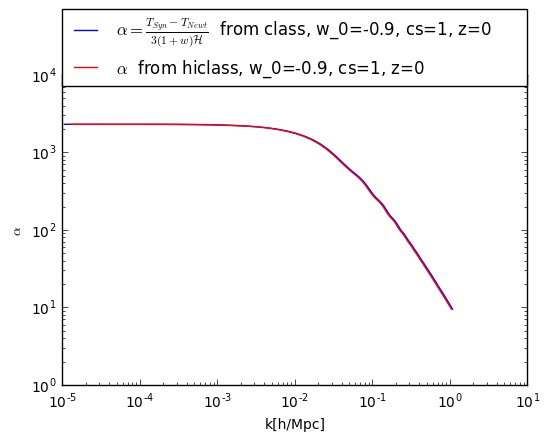
\includegraphics[width=0.60\textwidth]{alpha_class} 
\caption{The  $\alpha$ is in hi-class and class is compared. As it is clear they agree well. }
%\label{f1}
\end{center}
\end{figure}
%\begin{figure}[htbp!]
%\begin{center}
%\captionsetup{,margin=1cm}
%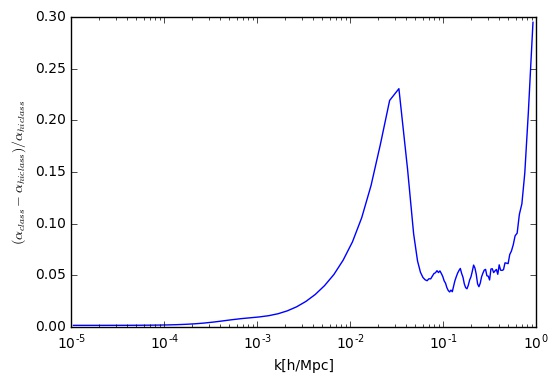
\includegraphics[width=0.60\textwidth]{alphaerror} 
%\caption{The  relative error of $\alpha$ in class and hi-class is shown. It is clear that  the relative error is very large in high wavenumbers.}
%%\label{plt2}
%\end{center}
%\end{figure}
\subsection{Comparing the  $\dot{\pi}$ transfer function directly from hi-class and EFTcamb and what we get from class indirectly}
We calculate field derivative transfer function in the class as following, since we know density contrast transfer function and $\Psi$ according to \ref{deltaeq} we can write,
\be
\pi'=\frac{c_s^2}{1+w} \delta_{newt} + \Psi 
\ee
The normalization factor in EFTcamb is assumed $\mathcal{H}$ and in class and hi-class the transfer function is assumed to be normalized to curvature function $\mathcal{R}$. So in the figure we have multiplied the EFTcamb result to $\mathcal{H}$ , hi-class and class result to $\delta_{\mathcal{R}}(k)= \frac{\sqrt{2 \pi^2 A_s(\frac{k}{k_p})^{n_s-1}}}{k^{3/2}}$.
\begin{figure}[H]
\begin{center}
\captionsetup{,margin=1cm}
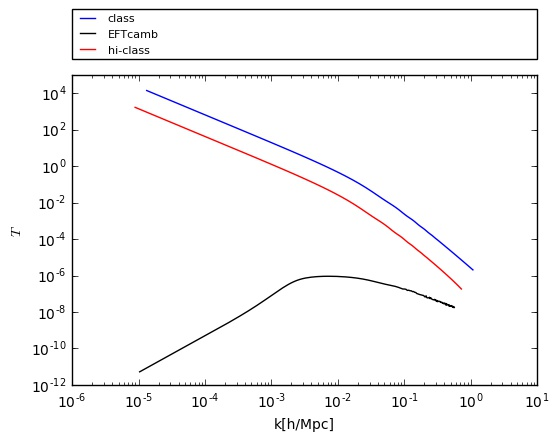
\includegraphics[width=0.60\textwidth]{field_derivative_comparison} 
\caption{Density contrast comparison in class and hi-class in Newtonian gauge.}
\label{plt2}
\end{center}
\end{figure}

\begin{figure}[H]
\begin{center}
\captionsetup{,margin=1cm}
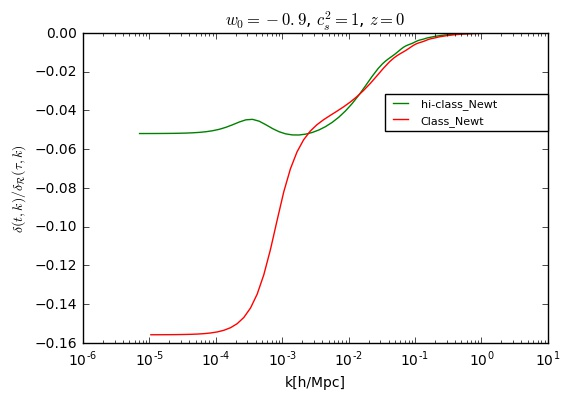
\includegraphics[width=0.60\textwidth]{newt_comp} 
\caption{Density contrast comparison in class and hi-class in Newtonian gauge.}
\label{plt2}
\end{center}
\end{figure}
\begin{figure}[H]
\begin{center}
\captionsetup{,margin=1cm}
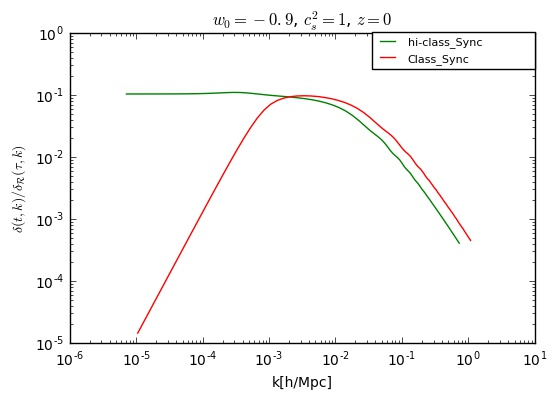
\includegraphics[width=0.60\textwidth]{sync_comp} 
\caption{Density contrast comparison in class and hi-class in Synchronous gauge. {\color{red}{which one is correct?!}}}
%\label{plt2}
\end{center}
\end{figure}
Now we try to compare the density transfer functions in the class and hi-class in two gauges,
\begin{figure}[H]
\begin{center}
\captionsetup{,margin=1cm}
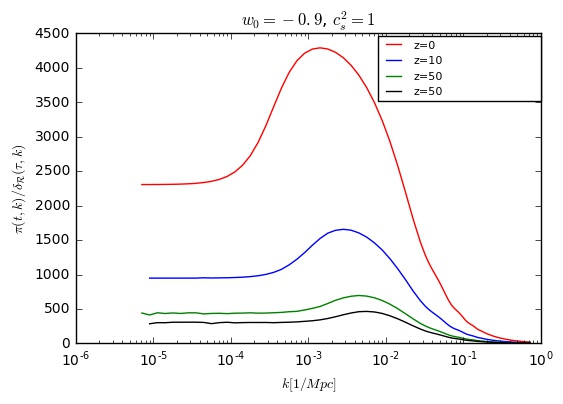
\includegraphics[width=0.60\textwidth]{pitransfer} 
\caption{Field transfer function in Newtonian gauge for quintessence model is plotted in different redshift}
%\label{plt2}
\end{center}
\end{figure}
\subsection{comparing the $\Psi$ function in Newtonian and synchronous gauge in class and hi-class}
Here we compare the metric fluctuation $\Psi$  in Newtonian gauge with one we obtain from Synchronous gauge parameters in class and hi-class codes to make sure we are dealing with the same functions. The $\Psi$ in Synchronous gauge reads as following,
\be
\Psi=\frac{1}{k^2} \Big [ {h^{''}}+ 6 {\eta^{''}} + \frac{a'}{a}  (h'+6 \eta ') \Big]= \alpha' + \mathcal{H}\alpha
\ee
In the figure \ref{psicomp} we compare the $\Psi$ in Newtonian gauge from what we get in terms of Synchronous gauge quantities.
\begin{figure}[H]
\begin{center}
\captionsetup{,margin=1cm}
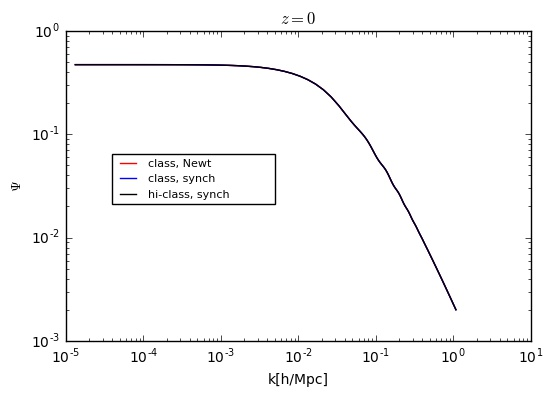
\includegraphics[width=0.60\textwidth]{psi_comp.jpg} 
\caption{$\Psi$ in Newtonian gauge and synchronous gauge in class and hi-class are compared. They all agree. }
\label{psicomp}
\end{center}
\end{figure}


\subsection{Test 2: Density transfer in the limit of $c_s^2 \rightarrow 0 , w \rightarrow -1$ which should be the same as matter density transfer function}
In the limit of zero sound speed and $w_0 \rightarrow -1$ we expect that the k-essence field behave like dark matter. In the fluid description in the class it can be seen easily. In the below figure the density contrast transfer function for k-essence fluid and dark matter fluid is plotted. \\
We expect the same behaviour for the obtained k-essence field from hi-class or EFTcamb. So a good criterion is checking the behaviour in the mentioned limit.
\begin{figure}[H]
\begin{center}
\captionsetup{,margin=1cm}
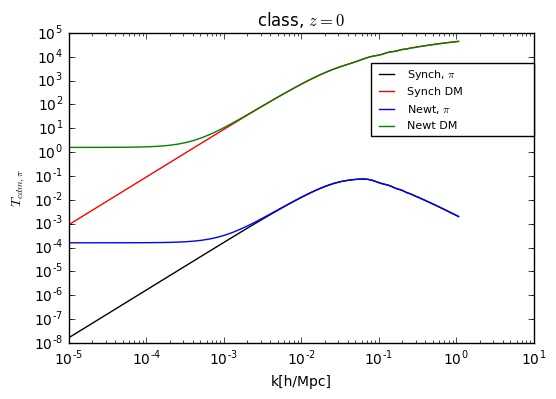
\includegraphics[width=0.60\textwidth]{cs0w1_fld.jpg} 
\caption{The behaviour of fluid and dark matter transfer function in the zero sound speed and $w_0 =-1$ limit is shown.  }
%\label{psicomp}
\end{center}
\end{figure}
Now we want to compare the result of density contrast transfer function of k-essence field in EFTcamb and hi-class with density contrast transfer of  fluid in the class.
The density constrast $\delta$ in the EFTcamb and hi-class is calculated,
\be
\delta=\frac{1+w_0}{c_s^2} (\pi'- \Psi) =10^4 (\pi'- \Psi)
\ee
As we have checked $\Psi$ is the same in Class and hi-class so we can use $\Psi$ to obtain the $\delta$ of EFTcamb as well.
\subsection{Comparison of $\dot{\pi}$ in hi-class from which we take from fluid description in the class}
First of all the relation between field in Synchronous gauge with the field in Newtonian gauge is given by:
\be
\pi_{New}=\pi_{Synch} + \alpha
\ee
\subsection{Comparison of field transfer functions in the hi-class and the EFTcamb}

\subsection{EFTcamb}
Now we want to use EFTcamb results for the quintessence which is straightforward to check the consistency of the result, \\
{\color{red} If we use pureEFT flag in EFTcamb, what are the related parameters for k-essence case?  since the translation between the standard language with EFTcamb is not trivial according to table 1 of   \url{https://arxiv.org/pdf/1411.3712.pdf} }
In the beginning we use minimally coupled quintessence flag in the EFTcamb to check the consistency, then we should try the pureEFT flag. We choose the quintessence flag according to \url{http://www.eftcamb.org/images/EFTCAMB_structure.pdf} in the second part.


\section{Gevolution}
All the transfer functions in the class and hi-class are normalized to one curvature perturbation. Curvature perturbation is obtained from powerspectrum as following,
\be
{\langle \mathcal{R} (k)  \mathcal{R} (k')\rangle} = (2 \pi )^3 \delta_D(k-k') P_{\mathcal{R}} (k)= (2 \pi )^3 \delta_D(k-k')  \frac{2 \pi^2}{k^3} \mathcal{P}_{\mathcal{R}}(k) =  (2 \pi )^3 \delta_D(k-k')   \frac{2 \pi^2}{k^3} A_s (\frac{k}{k_p})^{n_s-1}
\ee
So we can write
\be
\delta_{\mathcal{R}}(k)= \frac{\sqrt{2 \pi^2 A_s(\frac{k}{k_p})^{n_s-1}}}{k^{3/2}}
\ee
So $\delta_{\mathcal{R}}$, curvature perturbation transfer function, is the normalization factor which we should consider. Precisely we should multiply the field value from the class to $\delta_{\mathcal{R}}(k)$ to go in Gevolution units.\\
On the other hand, in the Gevolution after realization of the field the power spectrum is calculated as following,
\be
\langle \pi(k,t)  \pi(k,t) \rangle =(2 \pi )^3  P_{\pi} ^{Gev}=(2 \pi )^3   \delta_{\mathcal{R}}(k) ^2 P_{\pi}^{\text{hiclass}} = \frac{2 \pi^2}{k^3} A_s (\frac{k}{k_p})^{n_s-1} P_{\pi}^{\text{hiclass}}
\ee
In the Gevolution the wavenumber is measured in $\frac{h}{Mpc}$ but for the purpose of working with normal numbers it is multiplied to Boxsize so;
\be
k  \, \left[\frac{h}{Mpc} \right] = {k \times \text{Boxsize }}\, \left [\frac{{h}}{ \text{Boxsize }Mpc} \right]
\ee
As the powerspectrum in Gevolution in in $Mpc^3$ so $P(k[\frac{h}{Mpc}]) [\frac{Mpc^3}{h^3}]=P(k \, h [\frac{1}{Mpc}]) \left [{Mpc^3} \right ] $
%Plus in the gevolution $\frac{\text{Boxsize}}{Mpc}= \text{Number of grid points}$ 
The dimensionless powerspectrum is calculated as following: {(\color{red}{arXiv:0712.3028v2}}) \\
1- For the boxsize $L$, the field in Fourier space is discrete (no matter it is continuos or discrete in real space) and the k-modes are $\vec{k}= (\frac{2 \pi}{L}) (i,j,k)$. \\
2- The discrete Fourier transform is obtained by placing $\delta (x)$ on a lattice of  $N^3$ grid points with spacing $\frac{L}{N}$ 
\be
\delta_k^{DFT}= \frac{1}{N^3} \sum_r e^{-i\vec{k}.{r}} \delta(\vec{r})
\ee
3- Note that,
\be
\delta_k \approx ( \frac{\Delta x}{2 \pi} )^3 N^3 \delta_k^{DFT} \approx \dfrac{1}{\Delta k} \delta_k^{DFT} 
\ee
3- The powerspectrum is;
\be
P(k) \approx \frac{\langle | \delta^{DFT} |^2 \rangle}{(\Delta k)^3}
\ee
 4- The relation between dimensionless powerspectrum with the power with dimension is as following,
 \be
 \mathcal{P} (k)= \frac{k^3}{2 \pi ^2} P (k)
 \ee
 But factor $\frac{1}{N^6}$ should not be considered when we want to compare initial field transfer function with output powerspectrum! It is something internal in the Gevolution for calculating power from the realization. \\
 
-{\color{red}{Question:}} Why we do not get the same field realization (or order of magnitude) after going forward and backward in Fourier space? \\
- Is the below code right for realizing the field in Fourier and real space?
\begin{lstlisting}
generateRealization(*scalarFT_pi, 0., tk_d_kess, (unsigned int) ic.seed,
 ic.flags & ICFLAG_KSPHERE); 
plan_pi_k ->execute(FFT_BACKWARD);
pi_k->updateHalo();	// pi_k now is realized in real space
plan_pi_k->execute(FFT_FORWARD);}
\end{lstlisting}
If we turn off the following part we get completely different solution for the field in real space! As we expect the same order of magnitude of the $\pi (t,\vec{x})$ as other perturbations field $\phi$ so it seems we should turn off the below command! 
\begin{lstlisting}
plan_pi_k->execute(FFT_FORWARD); 
\end{lstlisting}
 
 \subsection{Some tests on Gevolution:}
 We want to test if the initial powerspectrum is the same as realized field powerspectrum in gevolution. \\
 In the figure \ref{comparehi-gev} the powerspectrum of the field from Gevolution's output is compared with the one which is made by hand. We make the dimensionless powerspectrum by hand from the initial transfer function as following,
 \be
 \mathcal{P}_{\pi}^{Gevolution} (k) = \frac{k ^3}{2 \pi ^2} \; \delta_{\mathcal{R}}^2 \,  \delta_{\pi}
^{\text{hiclass}} \times  \delta_{\pi}^{\text{hiclass}} =  \frac{k ^3}{2 \pi ^2} \;    \frac{2 \pi^2 A_s(\frac{k}{k_p})^{n_s-1}}{k^{3}}  \;  \delta_{\pi}
^{\text{hiclass}} \times  \delta_{\pi}^{\text{hiclass}} =    { A_s(\frac{k}{k_p})^{n_s-1}} \;  \delta_{\pi}
^{\text{hiclass}} \times  \delta_{\pi}^{\text{hiclass}} 
 \ee
 \begin{figure}[htbp!]
\begin{center}
\captionsetup{,margin=1cm}
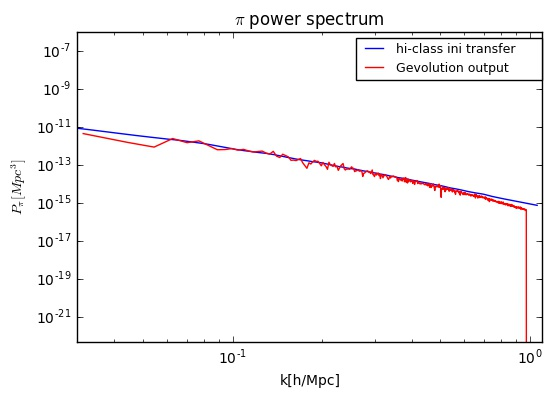
\includegraphics[width=0.60\textwidth]{Gev-hiclass} 
\caption{The powerspectrum which is calculated by hand is compared with output power of Gevolution. Simulation setting is: Boxsize=200 $Mpc/h$,  N$\_$grid=64 .  There is a deviation between two plots in high wavenumbers { \color{Red}{why?}}. While the Nyqvist frequency approximately is $\frac{2 \pi }{\Delta x} \approx  \frac{2 \pi \times \text{num}-{\text{grids}} }{\text{Boxsize}} =2.01 \, \frac{h}{Mpc}$}
\label{comparehi-gev}
\end{center}
\end{figure}
 
\section{Numerical solution to the k-essence equation }
The obtained equation from energy-momentum constraint $T^{\mu 0}_{;\mu}$ is written as below pertubatively;
\begin{align}
&-3 M_{pl}^2  \Omega_{kessence}  \Big [ 3 H^3 (w-1)-2 H \dot{H} \Big]  \epsilon^0   + 3 M_{pl}^2 H \Omega_{kessence} \Bigg[  -\Big(  (1+3w) H^2 +3 H \dot{w}    \nonumber \\&  +  2 (H^2 + \dot{H})(1+3 w)  \Big )  \Psi + \Big( -2\dot{H} (w+1)+H \dot{w}   \Big) \dot{\pi} - 3 H (1+w)\dot{ \Psi} + H (1+w) \frac{\nabla^2 \pi}{a^2} + H(1+w) \ddot{\pi} \Bigg] \epsilon \label{eq1}+ \mathcal{O}({\epsilon^2})=0
\end{align}


So, if we assume $\dot{w}=0$
\be
c^2 \frac{\nabla^2 \pi}{a^2} + \ddot{\pi} -3   \dot{\Psi} -\frac{(3 H^2+2 \dot{H}) (1+3 w) }{H (1+w)}  \Psi  - 2 H \dot{\pi} +  \frac{ 6H w}{ 1+w} \Phi =0 \label{eq2}
\ee

we take $d t=t_{n+1}-t_n $ and $x_{i,j,k} $ as lattice point,. We  solve the differential equation numerically as following;
\be
\pi_v= \dot{\pi}
\ee
\be
\pi^{n}= \pi ^{n-1}+\pi_v ^{n-\frac{1}{2}} d t
\ee
\be \label{eq3}
\pi_v ^{n+\frac{1}{2}}=\pi_v ^{n-\frac{1}{2}} + \ddot{\pi} ^{n}  d t 
\ee

From equation \ref{eq2} we have;
\begin{align}
& \ddot{\pi} ^{n} =- \frac{\pi^{n}_{i-1,j,k}+\pi^{n}_{i+1,j,k} +\pi^{n}_{i,j-1,k} +\pi^{n}_{i,j+1,k}+\pi^{n}_{i,j,k-1}+\pi^{n}_{i,j,k+1} -6 \pi^{n}_{i,j,k}  }{ a^2 dx^2}   +3 \frac{\Psi ^{n}_{i,j,k} -\Psi^{n-1}_{i,j,k} }{d t}    \nonumber \\ & + \frac{(3 H^2+2 \dot{H}) (1+3 w) }{H (1+w)} \Psi^{n}_{i,j,k} + H  \frac{(\pi_{v  \; {i,j,k}}^{n+\frac{1}{2}} +\pi_{v \; {i,j,k}}^{n-\frac{1}{2}} )}{2} -  \frac{ 6H w}{ 1+w} \Psi ^{n}_{i,j,k}
\end{align}
Where we have taken $\pi_{v  \; {i,j,k}}^{n} =\frac{(\pi_{v  \; {i,j,k}}^{n+\frac{1}{2}} +\pi_{v \; {i,j,k}}^{n-\frac{1}{2}} )}{2} $ \\
So we can rewrite the equation \ref{eq3} as below;
\begin{align} 
 &\pi_v ^{n+\frac{1}{2}}=\pi_v ^{n-\frac{1}{2}} +d t  \Big [c^2 \frac{\nabla^2 \pi ^n}{a^2} +3 \frac{\Psi ^{n}_{i,j,k} -\Psi^{n-1}_{i,j,k} }{d t} + \frac{(3 H^2+2 \dot{H}) (1+3 w) }{H (1+w)} \Psi^{n}_{i,j,k} + H  \frac{(\pi_{v  \; {i,j,k}}^{n+\frac{1}{2}} +\pi_{v \; {i,j,k}}^{n-\frac{1}{2}} )}{2} -  \frac{ 6H w}{ 1+w} \Phi ^{n}_{i,j,k} \Big]
\end{align}
So the set of equations we should solve are;
\begin{align} 
 \pi_v ^{n+\frac{1}{2}}= & \frac{1}{1- dt H/2} \Bigg[ (1+ dt H/2)\pi_v ^{n-\frac{1}{2}} + c^2 d t  \Big (  \frac{\pi^{n}_{i-1,j,k}+\pi^{n}_{i+1,j,k} +\pi^{n}_{i,j-1,k} +\pi^{n}_{i,j+1,k}+\pi^{n}_{i,j,k-1}+\pi^{n}_{i,j,k+1}  -6 \pi^{n}_{i,j,k}  }{ a^2 dx^2}  \nonumber \\ & +3 \frac{\Psi ^{n}_{i,j,k} -\Psi^{n-1}_{i,j,k} }{d t} + \frac{(3 H^2+2 \dot{H}) (1+3 w) }{H (1+w)} \Phi^{n}_{i,j,k} -  \frac{ 6H w}{ 1+w} \Phi ^{n}_{i,j,k} \Big) \Bigg]
\end{align}
\be
\pi^{n+1}= \pi ^{n}+\pi_v ^{n+\frac{1}{2}} d t
\ee
Then we need to calculate $\dot{H}$ and $\dot{\Psi}$ in each loop. \\
To calculate $\dot{\Psi}$ we save two $\Psi$ in each loop. \\
 On the other hand we have $\dot{H}$ according to the background constraint of Energy-momentum tensor divergence according to eq.\ref{eq1},
\be
-3 M_{pl}^2  \Omega_{kessence}  \Big [ 3 H^3 (w-1)-2 H \dot{H} \Big]  \epsilon^0 =0
\ee
\be
\dot{H}_{(n)}= \frac{3}{2} H^2 _{(n)} (w-1)
\ee
Gevolution works with conformal time $\tau$ and light velocity equal to one $c=1$, which imposes 
\section{Programming issues}
One the programming issue is related to the fact that we want to separate background updates of the particles with background updates of the k-essence field. We define another scale factor in the code "a-kess" which takes the value of the scale factor, then it updates the field. In order to match the two background scale factor, we must pay the cost that in the first loop the velocity field is updated only by half step not more. If we want to break the half step updating into some sub steps, it does not work, since the background for particles update are not updated by half step in the first loop! So two scale factors mismatch. \\
Moreover because we calculate the field derivative in half step using the scale factor in previous half step, we have an error relating to the fact that the velocity field is constructed from the scale factor in different time! \\
The procedure is explained as following,
\begin{lstlisting}
if(cycle==0)
{
	update_pi_k_v( 0.5 * dtau);
	rungekutta4bg(a_kess, fourpiG, cosmo,  0.5 * dtau  );
	pi_k.updateHalo();
	pi_v_k.updateHalo();
}

else
{
	for (i=0;i<sim.nKe_numsteps;i++)
	{
		update_pi_k( dtau  / sim.nKe_numsteps);
		update_pi_k_v( dtau  / sim.nKe_numsteps);
		rungekutta4bg(a_kess, fourpiG, cosmo,  dtau  / sim.nKe_numsteps);
		pi_k.updateHalo();
		pi_v_k.updateHalo();
	}
}
\end{lstlisting}
%\be
% \ddot{\pi} ^{n} =- \frac{\nabla^2 \pi}{a^2} + \ddot{\pi} +3   \dot{\Phi} -\frac{(3 H^2+2 \dot{H}) (1+3 w) }{H (1+w)}  \Phi  - 2 H \dot{\pi} +  \frac{ 6H w}{ 1+w} \Psi 
%\ee
%\begin{align}
%& \frac{\pi^{n}_{i-1,j,k}+\pi^{n}_{i+1,j,k} +\pi^{n}_{i,j-1,k} +\pi^{n}_{i,j+1,k}+\pi^{n}_{i,j,k-1}+\pi^{n}_{i,j,k+1} -6 \pi^{n}_{i,j,k}  }{ a^2 dx^2} -  \frac{\pi^{n+1} _{i,j,k} - \pi ^{n}_{i,j,k}  + \pi ^{n-1}_{i,j,k}  }{dt ^2}\nonumber \\ &  -3 \frac{\Phi ^{n+1}_{i,j,k} -\Phi^{n}_{i,j,k} }{d t} - \frac{(3 H^2+2 \dot{H}) (1+3 w) }{H (1+w)} \Phi^{n}_{i,j,k} -2 H  \frac{(\pi_{v  \; {i,j,k}}^{n+1} -\pi_{v \; {i,j,k}}^{n-1} )}{dt} +  \frac{ 6H w}{ 1+w} \Psi ^{n+1}_{i,j,k}
%\end{align}
%What I think;
%\begin{align}
%& \frac{\pi^{n}_{i-1,j,k}+\pi^{n+1}_{i+1,j,k} +\pi^{n+1}_{i,j-1,k} +\pi^{n+1}_{i,j+1,k}+\pi^{n+1}_{i,j,k-1}+\pi^{n+1}_{i,j,k+1} -6 \pi^{n+1}_{i,j,k}  }{dx^2} -  \frac{\pi^{n+1} _{i,j,k} - \pi ^{n}_{i,j,k}  + \pi ^{n-1}_{i,j,k}  }{dt ^2}\nonumber \\ &  -3 \frac{\Phi^{n}_{i,j,k} }{d t} - \frac{(3 H^2+2 \dot{H}) (1+3 w) }{H (1+w)} \Phi^{n}_{i,j,k} -2 H  \frac{(\pi_{v  \; {i,j,k}}^{n+1/2} -\pi_{v \; {i,j,k}}^{n-1/2} )}{dt} +  \frac{ 6H w}{ 1+w} \Psi ^{n+1}_{i,j,k}
%\end{align}
\begin{appendices}
\section{Derivative of determinant} \label{A1}
Assume an invertible matrix M,
\be
\det\left( M+\delta M \right) =\det \left( M\left( 1+M^{-1}\delta M\right) \right)
\ee
where $\delta M$ is a small change in the matrix M. According to the properties of determinant $\det\left( AB\right) =\det\left( A\right) \det\left( B\right) 
$ we have,
\be
\det\left( M\left( 1+\delta M\right) \right) =\det M\det\left( I+\delta M\right) 
\ee
%According to Cayley-Hamilton theorem: \\
For a $n \times n$ matrix M, the characteristic polynomial is defined by p($\lambda$)=$\det (A- \lambda I)$=$(-1)^n \Big[ \lambda ^n +c _1 \lambda ^{n-1} + c _2 \lambda ^{n-2}  +...+c_n \Big]$  where $c_n=(-1)^n \det( A)$, $c_1=tr (A)$. So,
\be
\det\left( I+\delta M\right) =p(\lambda=1)=1^{n}+1^{n-1}tr\left( \delta M\right) +O\left( \delta M^{2} \right) 
\ee
On the other hand,
\begin{align}
\delta\det M&=\det\left( M+\delta M\right) -\det\left( M\right) =\det M\det\left( I+\delta M\right) -\det\left( M\right) \nonumber \\ &
=\det M (1+ tr(\delta M)) -\det\left( M\right)= \det M  \, tr (\delta M)
\end{align}
So for the metric we can write the same statement to get the result,
\be
\delta g =\delta \det g_{\mu \nu}=  \det (g_{\mu \nu}+ \delta g_{\mu \nu}) - \det (g_{\mu \nu}) = \det (g_{\mu \nu}) tr (\delta g_{\mu \nu}) = g \, \delta g_{\mu\nu}g^{\mu\nu}
\ee
Pay attention to the relation between $\delta g^{\mu \nu}$ and $\delta g_ {\mu \nu}$ which shows that $\delta g_{\mu \nu}$ is not a tensor!
\be
g_{\mu\nu}g^{\nu\rho}=\delta^{\rho}_{\mu} \rightarrow
\delta g_{\mu\nu}g^{\nu\rho}+g_{\mu\nu}\delta g^{\nu\rho}=0 
\ee
\be
\delta g^{\nu\rho}=-g^{\nu\sigma}\delta g_{\sigma\mu}g^{\mu\rho}
\ee
\end{appendices}

\end{document}

 